\chapter{PLP algorithm}\label{ap:plp}
The PLP algorithm such as it was implemnted in this work and developed by \citet{plp}.


\makeatletter
\def\BState{\State\hskip-\ALG@thistlm}
\makeatother

\begin{algorithm}
\caption{PLP algorithm}

\begin{algorithmic}

\State $ \textbf{U} \gets \text{Set of vertices of type A}$
\State $ \textbf{V} \gets \text{Set of vertices of type B}$
\State $ \textbf{E} \gets \text{Set of edges}$
\State $ \textbf{G} \gets \text{Graph }\textbf{G}=(\textbf{U},\textbf{V},\textbf{E})$

\State /* Construct the set of all patterns */

\State $ \textbf{E}_u \gets \emptyset$
\For{each node in B in \textbf{U}}
    \For{each node x in \textbf{N}(B)}
        \For{each node in C in \textbf{N}(x)}
            \State $\textbf{E}_u \gets \textbf{E}_u \cup \{(B,C)\}$
        \EndFor
    \EndFor
\EndFor

\State /* Calculate the weight of each pattern */

\For{each edge (B,C) in $\textbf{E}_u$}
    \State Calculate the weight for pattern (B,C)
\EndFor

\State /* Calculate the connectivity of CNPs */

\For{each node B in projected graph $\textbf{G}_u$}
    \For{each neighbor C of B in projected graph $\textbf{G}_u$}
        \For{each node x linked with C in \textbf{G}}
            \If{(B,x) $\notin$ \textbf{E}}
                \State S(B,x) = S(B,x) + w(B,C)
            \EndIf
        \EndFor
    \EndFor
\EndFor

\State /* Output the connectivity of the CNPs in matrix S.

\end{algorithmic}
\end{algorithm}

\newpage

\chapter{Extraction to Graph Database}\label{ap:query}
Below in Listing \ref{lst:query} an example query that builds a database with the nodes
\begin{itemize}
    \item IpAddress
    \item Malware
    \item MalwareCategory
    \item CyberVulnerability
    \item Hash
    \item EmailAddress
    \item InternetDomainName
    \item AttackVector
    \item Product
\end{itemize}
and the relations connecting the nodes
\begin{itemize}
    \item $IpAddress->[RELATED\_TO]->IpAddress$
    \item $IpAddress->[RELATED\_TO]->Malware$
    \item $IpAddress->[RELATED\_TO]->MalwareCategory$
    \item $IpAddress->[RELATED\_TO]->CyberVulnerability$
    \item $IpAddress->[RELATED\_TO]->Hash$
    \item $IpAddress->[RELATED\_TO]->EmailAddress$
    \item $IpAddress->[RELATED\_TO]->InternetDomainName$
    \item $IpAddress->[RELATED\_TO]->AttackVector$
    \item $IpAddress->[RELATED\_TO]->Product$
\end{itemize}

This query was later combined with queries where the IpAddress was replaced with Cybervulnerability and the other node types. In this additive way the data set used for classification of malicious ip address was built.

A sample of the resulting graph is shown in \figref{fig:qdb}.

\begin{figure}
    \centering
    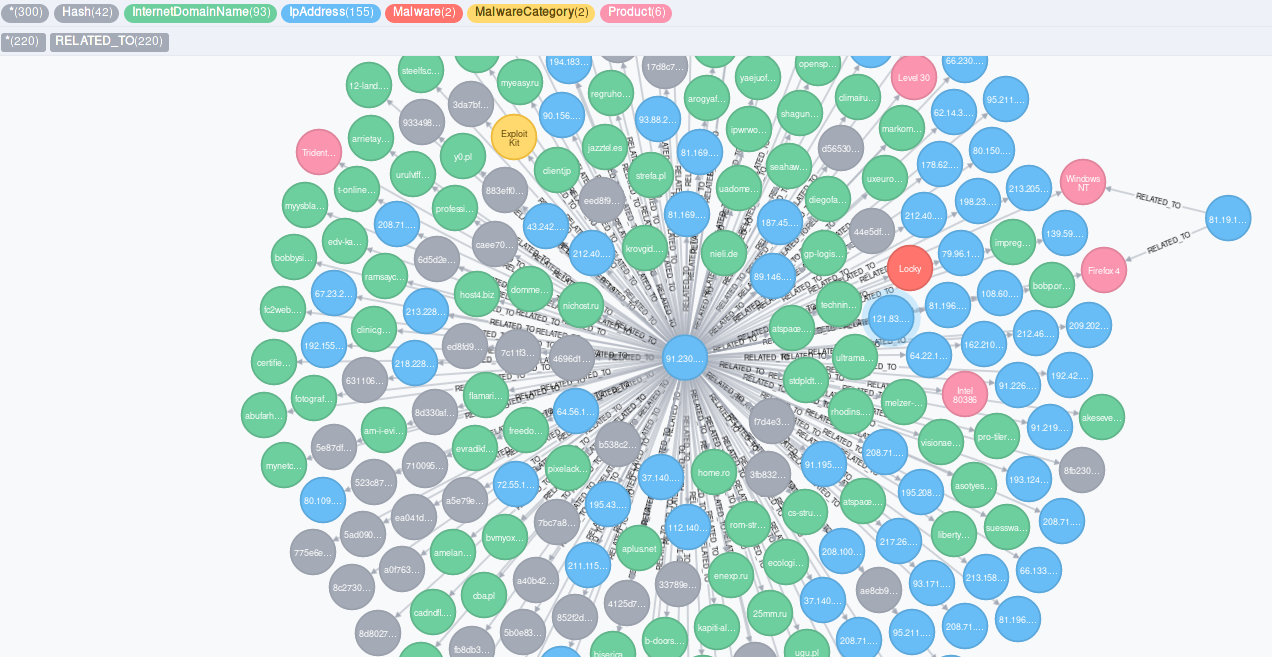
\includegraphics[width=\textwidth]{images/neo_ex_q.png}
    \caption{Caption}
    \label{fig:qdb}
\end{figure}

\lstinputlisting[caption=Example query for extracting nodes and relations from Recorded Future API,label=lst:query]{query_example.txt}